Les couches morphologiques, telles que décrites précédemment, sont intégrées dans les réseaux de neurones morphologiques de la même manière que les couches de convolution dans les réseaux de neurones convolutionnels \cite{Hassoun_1996}. Dans le cadre de ce travail, nous construisons des réseaux comportant uniquement une ou plusieurs couches morphologiques successives, et pouvant comporter en plus (ou non) des couches de rééchelonnage de l'image, constantes ou avec des poids variables appris par le réseau lors de la phase d'entraînement, telles qu'une couche de convolution de taille 1 \cite{Keiller_2019, Bloch_2021}. \\

\vspace{-0.6mm}
\noindent Dans un tel réseau morphologique :
\vspace{0.8mm}
\begin{itemize}%[leftmargin=*]
    \item[$\bullet$] l'entrée est une matrice 3D représentant un ensemble d'images 2D en niveaux de gris définies sur une partie $I$ de $\mathbb{Z}^2$, de taille $n \times l \times h$, avec $n$ le nombre d'images, $l$ la longueur verticale des images et $h$ leur hauteur ;
    \vspace{0.4mm}
    \item[$\bullet$] les images sont filtrées successivement par les différentes couches du réseau, à travers une succession ordonnées de couches morphologiques et de couches de rééchelonnage si incluses dans le réseau ;
    \vspace{0.4mm}
    \item[$\bullet$] la sortie est une matrice 3D représentant l'ensemble des $n$ images 2D filtrées, de même taille $n \times l \times h$ que la matrice d'entrée. \\
\end{itemize}

\vspace{-1.0mm}
Le nombre de couches morphologiques à intégrer dans ces réseaux dépend de l'opération que l'on souhaite simuler ou du contexte dans lequel ils s'inscrivent. \\

\vspace{-1.6mm}
\noindent Typiquement, pour des opérations d'érosion ou de dilatation, le réseau comportera une unique couche morphologique, accompagnée ou non de couches de rééchelonnage. Pour des opérations d'ouverture (érosion suivie de dilatation) ou de fermeture (dilatation suivie d'érosion), chaque couche morphologique ne pouvant simuler le comportement que de l'une des deux opérations morphologiques fondamentales, le réseau comportera deux couches morphologiques successives, dans le but que l'une simule le comportement d'une érosion, et que l'autre simule celui de l'érosion. Pour une opération de dessalage (i.e. supprimer les bruits poivre et sel sur les images), on voudra intégrer quatre couches morphologiques successives, pour tenter d'imiter le comportement d'une ouverture suivie d'une fermeture, ou inversement. \\

\vspace{-1.6mm}
\noindent Il sera également possible de construire des réseaux comportant plusieurs couches morphologiques, dans le cadre d'une simple opération d'érosion ou de dilatation, afin de mieux comprendre leur fonctionnement et d'étudier le comportement et la convergence de ces réseaux durant la phase d'apprentissage. Un des points d'intérêt est l'étude de la forme que les noyaux adopteront pour décomposer en plusieurs parties une opération qu'une seule couche suffit à simuler. A l'inverse, il pourra être également pertinent d'étudier le comportement de réseaux composés d'une seule couche, pour des opérations plus complexes que l'érosion ou la dilatation.


\newpage

% figure
\begin{figure}[ht]
  \begin{center}
    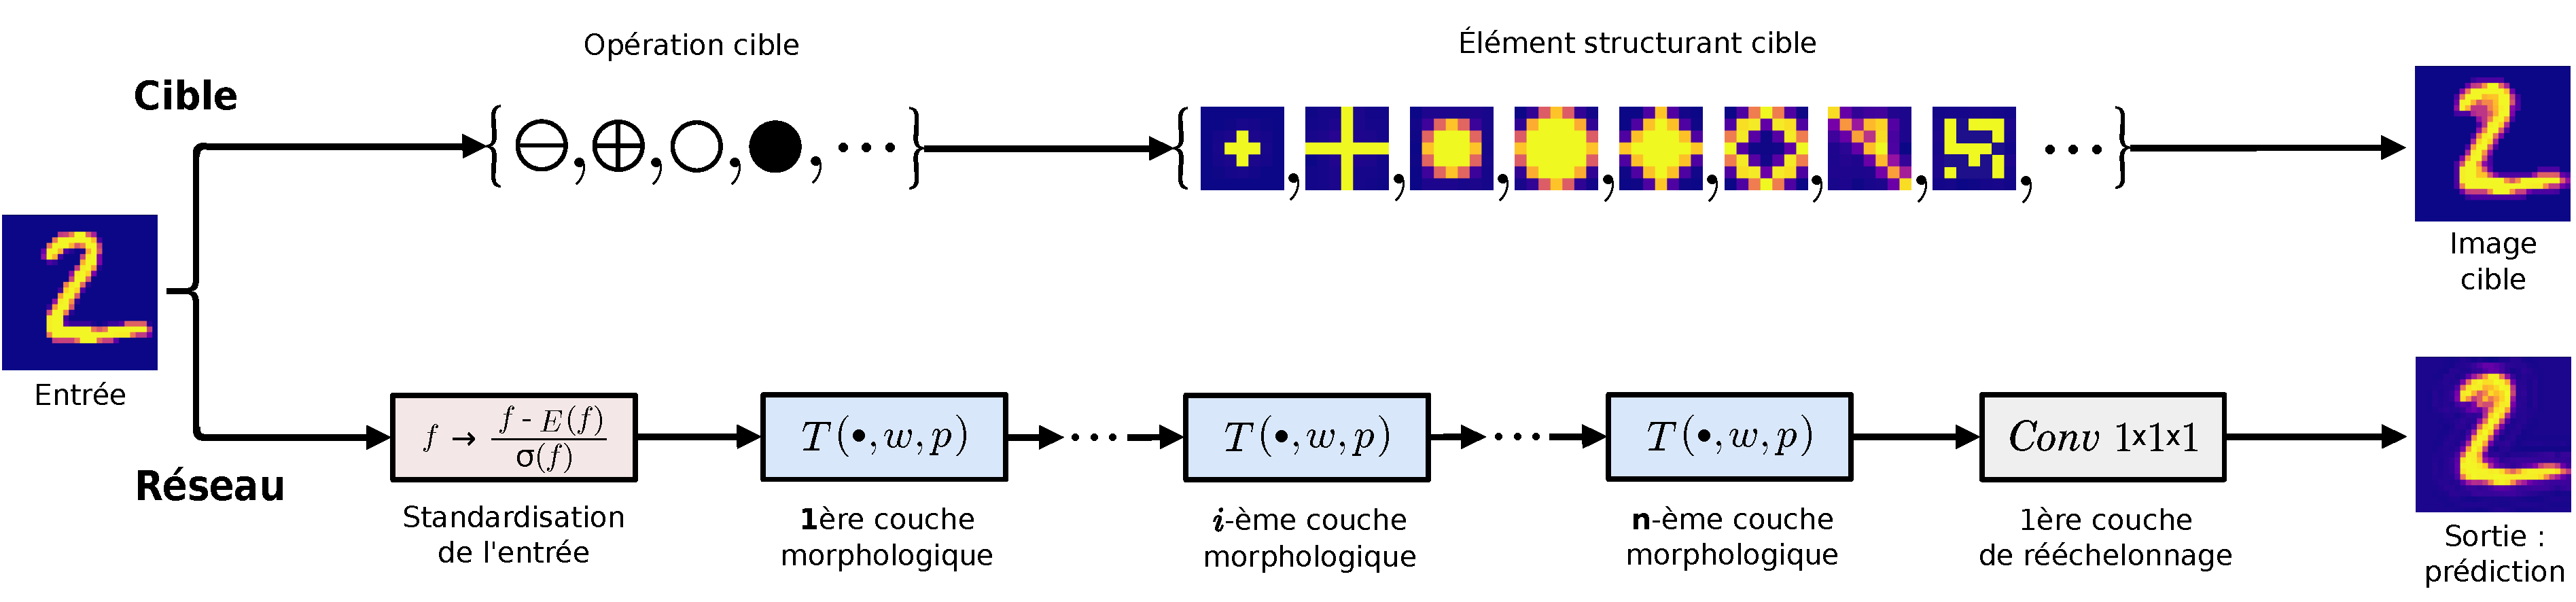
\includegraphics[width=1.00\textwidth]{parts/2-etat_de_lart/B-structure_des_reseaux_morphologiques/figures/reseau_morpho.pdf}
    \vspace{-3.6mm}
    \caption{ \centering Illustration de l'architecture type des réseaux de neurones morphologiques. Cas où l'opération et l'élément structurant cibles sont définis.}
    \label{fig:architecture_reseau_morpho}
  \end{center}
\end{figure}

\vspace{-3.4mm}
De plus, l'intégration ou non de couches de rééchelonnage des valeurs des images dépend des besoins et du comportement de convergence du réseau. Un filtre de rééchelonnage peut être linéaire (normalisation linéaire dans un intervalle $[a,b]$, standardisation, etc.) ou de forme plus complexe (logarithmique, tangente hyperbolique, etc.), et peut être constant (fonction déterministe invariante) ou comportant des poids variables appris par le réseaux lors de l'apprentissage. Dans ce dernier cas, les filtres linéaires sont typiquement de la forme : $f \rightarrow f \times s + b$, avec $s$ l'échelle (<< scale >>) et $b$ le biais (<< bias >>), tous deux formant les deux poids de cette couche de rééchelonnage. Il s'agit donc d'une couche de convolution classique, de taille $1 \times 1 \times 1$. \\

\vspace{-2.2mm}
%Pour des raisons d'amélioration de la convergence, plusieurs opérations intermédiaires, en entrée du réseau, entre les couches morphologiques, ou en sortie du réseau, peuvent être faites sur les images. En particulier, 
Hermary et al. \cite{Hermary_2022} ont montré que l'ajout d'un filtre de standardisation des images en entrée du réseau, accompagnée d'une couche de rééchelonnage linéaire de l'image (convolution) en sortie de ce dernier, permet une meilleure convergence lors de la phase d'apprentissage. 
Ainsi, l'architecture type des réseaux de neurones morphologiques qu'on utilisera est illustrée fig \ref{fig:architecture_reseau_morpho}. Elle définit d'abord un filtre de standardisation des images, puis $n$ couches morphologiques successives, pour finir avec une couche de convolution de taille 1 pour rééchelonner l'image en sortie. L'illustration montre le cas où l'opération et l'élément structurant cibles sont définis. Mais ils peuvent ne pas l'être, comme dans le cas du dessalage, où l'on considère simplement des images cibles vers lesquelles les prédictions du réseau cherchent à converger. \\

\vspace{-2.2mm}
A noter que le réseau construit n'est informé ni de l'opération cible, ni de l'élément structurant cible. Le réseau converge librement et se met à jour uniquement par rapport à l'image de sortie cible ; les poids (les $w_i$ du noyau $w$ et le paramètre de contrôle $p/\alpha$) des couches morphologiques et ceux des couches de rééchelonnage se mettant à jour sur la base de l'erreur (MSE) entre l'image cible et l'image prédite par le réseau. Ainsi, les couches morphologiques ne convergent pas nécessairement vers l'état espéré, et chacun n'adopte pas forcément un comportement morphologique (soit érosion ou soit dilatation) tel que souhaité, dû au lissage continue obligatoire de la transition entre un comportement d'érosion ou de dilatation de la couche. Là est tout l'enjeu d'une bonne définition de la fonction de transformation $T$ des couches et de l'analyse du comportement et de la convergence des réseaux construits.
